\documentclass[12pt]{article}

\usepackage{sbc-template}
\usepackage{graphicx,url,amssymb,hyperref}
\usepackage[utf8]{inputenc}
\usepackage[english]{babel}
\usepackage[T1]{fontenc}

\sloppy

\title{A comparison between the usage of free and proprietary solutions for General-purpose computing on GPUs (GPGPU)}

\author{Isabella B. do Amaral\inst{1}, Alfredo G. vel Lejbman\inst{2}}


\address{University of São Paulo (USP)\\
  São Paulo, SP -- Brazil
  \email{isabellabdoamaral@usp.br}
\nextinstitute
  Mathematics and Statistics Institute (IME) -- University of São Paulo (USP)\\
  São Paulo, SP -- Brazil
  \email{gold@ime.usp.br}
}

\begin{document}

\maketitle

\begin{abstract}
    In this research project, we explore the usage of open-source and proprietary
    solutions for performing general-purpose computing on graphics processing
    units (GPGPU).
    We begin by analyzing project statistics and categorizing them according to
    their descriptions using unsupervised machine learning.
    Then, we compare the performance and usability of the solutions, proposing
    enhancements to better support the development of open-source GPGPU
    tooling.
\end{abstract}

\section{Introduction} \label{sec:intro}

\subsection{Motivation} \label{sec:intro:motivation}

Computers have become invaluable assets to research, mainly with respect to
numerical problems that are largely unsolvable through analytical methods.
As needs evolve, not only software but also hardware has become increasingly
complex, giving rise to what we call \textbf{heterogeneous systems}.
These systems are composed of multiple processing units, each with its own
architecture, which will dictate performance characteristics for different
workloads.

Graphics Processing Units (GPUs) are optimized for parallel computation, which
works by taking advantage of uncoupled data, and can cut execution times
proportionally to the number of computational units available.
Linear algebra routines, which can be thoroughly optimized for parallelism, sit
at the core of many scientific applications, such as machine learning and
numerical simulations.
We can clearly see that GPUs outperform CPUs in such tasks, as shown in
\cite{buber2018performance}.

Unfortunately, software for research does not seem to be held to standards as
high as more traditional content (see \cite{sufi2014software}).
It is also often developed by researchers that are inexperienced in real
world development practices, leading to unmaintainable code (see
\cite{carver2022survey}).

One particular development strategy that appeals to modern scientific standards
is that of open source, in which the code is fully available to the public.
Most obviously, as open-source software is auditable, it becomes easier to
verify the reproducibility of scientific results created with it (see
\cite{barba2022defining}), but this also allows for early collaboration between
researchers and developers, which can lead to better software design and
performance (see \cite{wilson2014best}).

Building on the practice of open source we also have \textit{free software}
(commonly denoted by FLOSS or FOSS): a development ideology that focuses around
volunteer work and donations, criticizing corporate interests, and is usually
accompanied by permissive or \textit{copyleft} licenses.
There is emerging work on the role of FLOSS in science, such as
\cite{fortunato2021case}, and some initiatives which praise a similar approach
(see \cite{katz2018community, barker2022introducing}).

\subsection{Proposal} \label{sec:intro:proposal}

As the GPU is a separate piece of hardware, it is necessary to use specialized
APIs to communicate with it.
Implementation of such APIs is usually provided by the hardware vendor, as it
depends on the specific architecture of the GPU.
Graphics APIs provide much-needed abstractions to the programmer, as they are
made to orchestrate the entire pipeline, making the choice of API a crucial
decision for the robustness of a given application.

In the context of GPGPU, \textbf{CUDA} -- a proprietary API
projected and maintained by NVIDIA -- is historically significantly more
widespread than any other API, proprietary or not.
On the one hand, most open-source alternatives that provide the same
functionality are either in their infancy or have not provided what was needed
to replace CUDA, examples are, respectively, HIP by AMD, and OpenCL by the
Khronos Group.
On the other hand, OpenCL-related tooling has recently gained more focus
amongst open-source software consultancies, as we can see in
\cite{Nicola_2022}, so it is possible that the situation is changing.

Thus, in this research project, we aim to:
\begin{enumerate}
    \item\label{obj1} Get a more precise figure of the usage of
        graphics-accelerated open-source software used in scientific
        applications.
    \item\label{obj2} Find out how CUDA stands out from open-source
      alternatives.
    \item\label{obj3} Find ways to overcome such differences and make it easier
        for maintainers to add support for open-source APIs.
\end{enumerate}

We choose to analyze \textbf{Vulkan} and \textbf{OpenCL} as they are the most
prominent open-source alternatives to CUDA, and we will also take a look at
\textbf{HIP} as it is the most recent addition to the list.
Both Vulkan and OpenCL are Khronos Group standards, of which more than 170
companies are members, including AMD, ARM, Intel, NVIDIA, and Qualcomm.
Their API specifications are open and have ample documentation and adoption,
which makes them a good choice for our analysis.
HIP (Heterogeneous-Compute Interface for Portability) provides a solution to
ease the transition from CUDA to more portable code, thus making it interesting
to us as well.

\section{Methodology} \label{sec:methodology}

So far, we have made some progress on \ref{obj1} by analyzing popular
graphics-accelerated projects using topic modeling\footnote{
    All code related to this work is available at \href{https://github.com/isinyaaa/foss-gpgpu-stack}{isinyaaa/foss-gpgpu-stack}.
}.

\subsection{Data collection} \label{sec:methodology:data-collection}

We assume that most relevant scientific applications have support for CUDA.
\href{https://nvidia.com/en-us/gpu-accelerated-applications}{NVIDIA's list of accelerated apps}
provides a non-exhaustive list of (somewhat relevant) applications that use
it, and by filtering by relevant categories and manual sorting, we got a list of 141 projects that
are open source and use \verb|git| as their version
control system.
After that, following \cite{zheng2018measuring}'s methodology, we gathered the
repositories' \verb|README| files and removed sections that were not relevant to
our analysis.

\subsection{Data analysis} \label{sec:methodology:data-analysis}

The gathered data was cleansed further, removing stop words, symbols (such as
punctuation), standalone numbers, and very short words.
We then break up the data into sizeable chunks by tokenizing and lemmatizing
it.
This reduces the number of words to a more
manageable amount, and also makes it allows us to compare words that are similar
in meaning.

We then store the results of preprocessing in a count vector so that we can
abstract away from the order of the words, thus making it easier to compare
documents.
In this step, we also remove words that appear in less than $10\%$
of documents, or in more than $90\%$ of them, as they are either
too common or too rare to be relevant to the analysis.

After that, we use Latent Dirichlet Allocation (LDA) to group the documents
into $N$ topics.
We use the \textit{coherence score} for tuning the hyperparameters of our
model, randomizing samples of the data so we don't overfit the model to the data
while testing for different ranges of hyperparameters with varying precision.

We were able to generate clear visualizations for a tuned \verb|gensim| model by using the
\textit{t-distributed stochastic neighbor embedding} (t-SNE) method for
\verb|pyLDAvis|, as we can see in
\ref{fig:lda_gensim_tsne}.
T-SNE works well with sparse data, as it is better able to preserve local
structure, but it needs manual tuning.

\begin{figure}[ht]
    \centering
    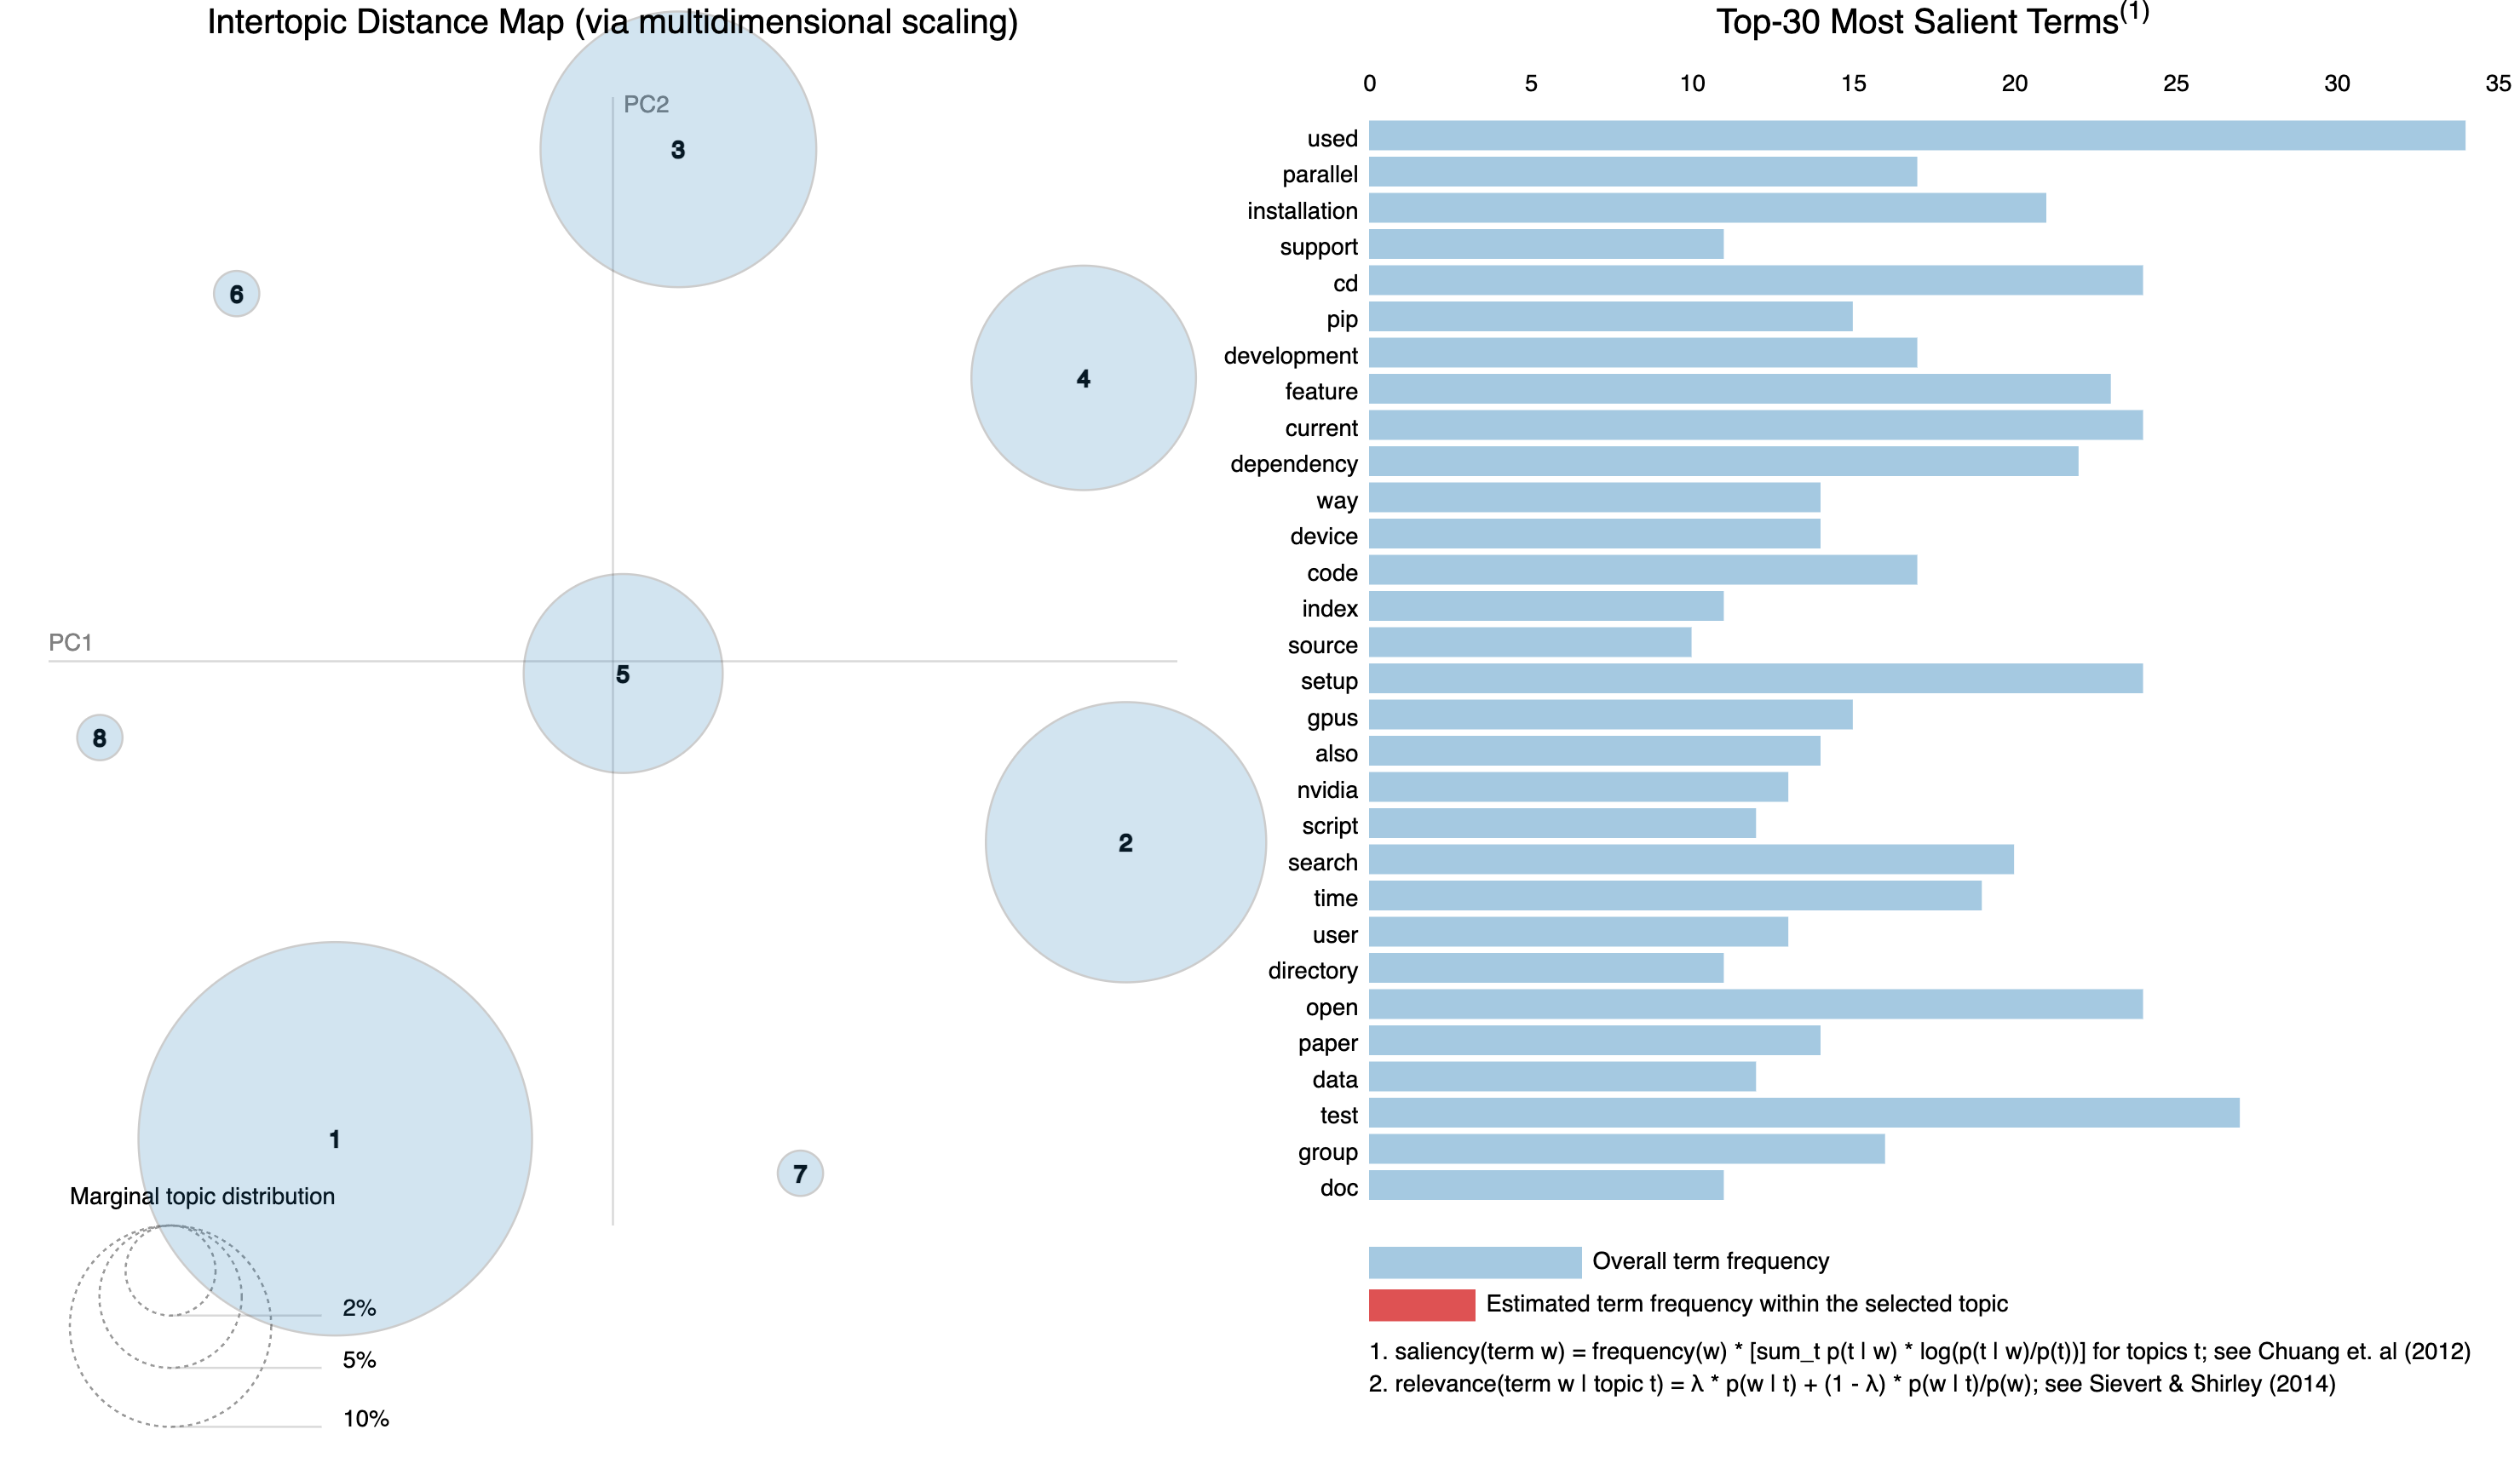
\includegraphics[width=\linewidth]{gensim-tsne.png}
    \caption{Visualization of gensim's LDA results (trained model with t-SNE
        dimensionality reduction method).}
    \label{fig:lda_gensim_tsne}
\end{figure}

\section{Discussion} \label{sec:discussion}

By taking the most likely topic for each document, we were able to plot
\ref{fig:topic-probabilities}.
Looking at the words composing each topic, it's still non-trivial to label
them, thus we are still unable to make any conclusions about the
repositories' actual subjects, requiring further analysis.

\begin{figure}[ht]
    \centering
    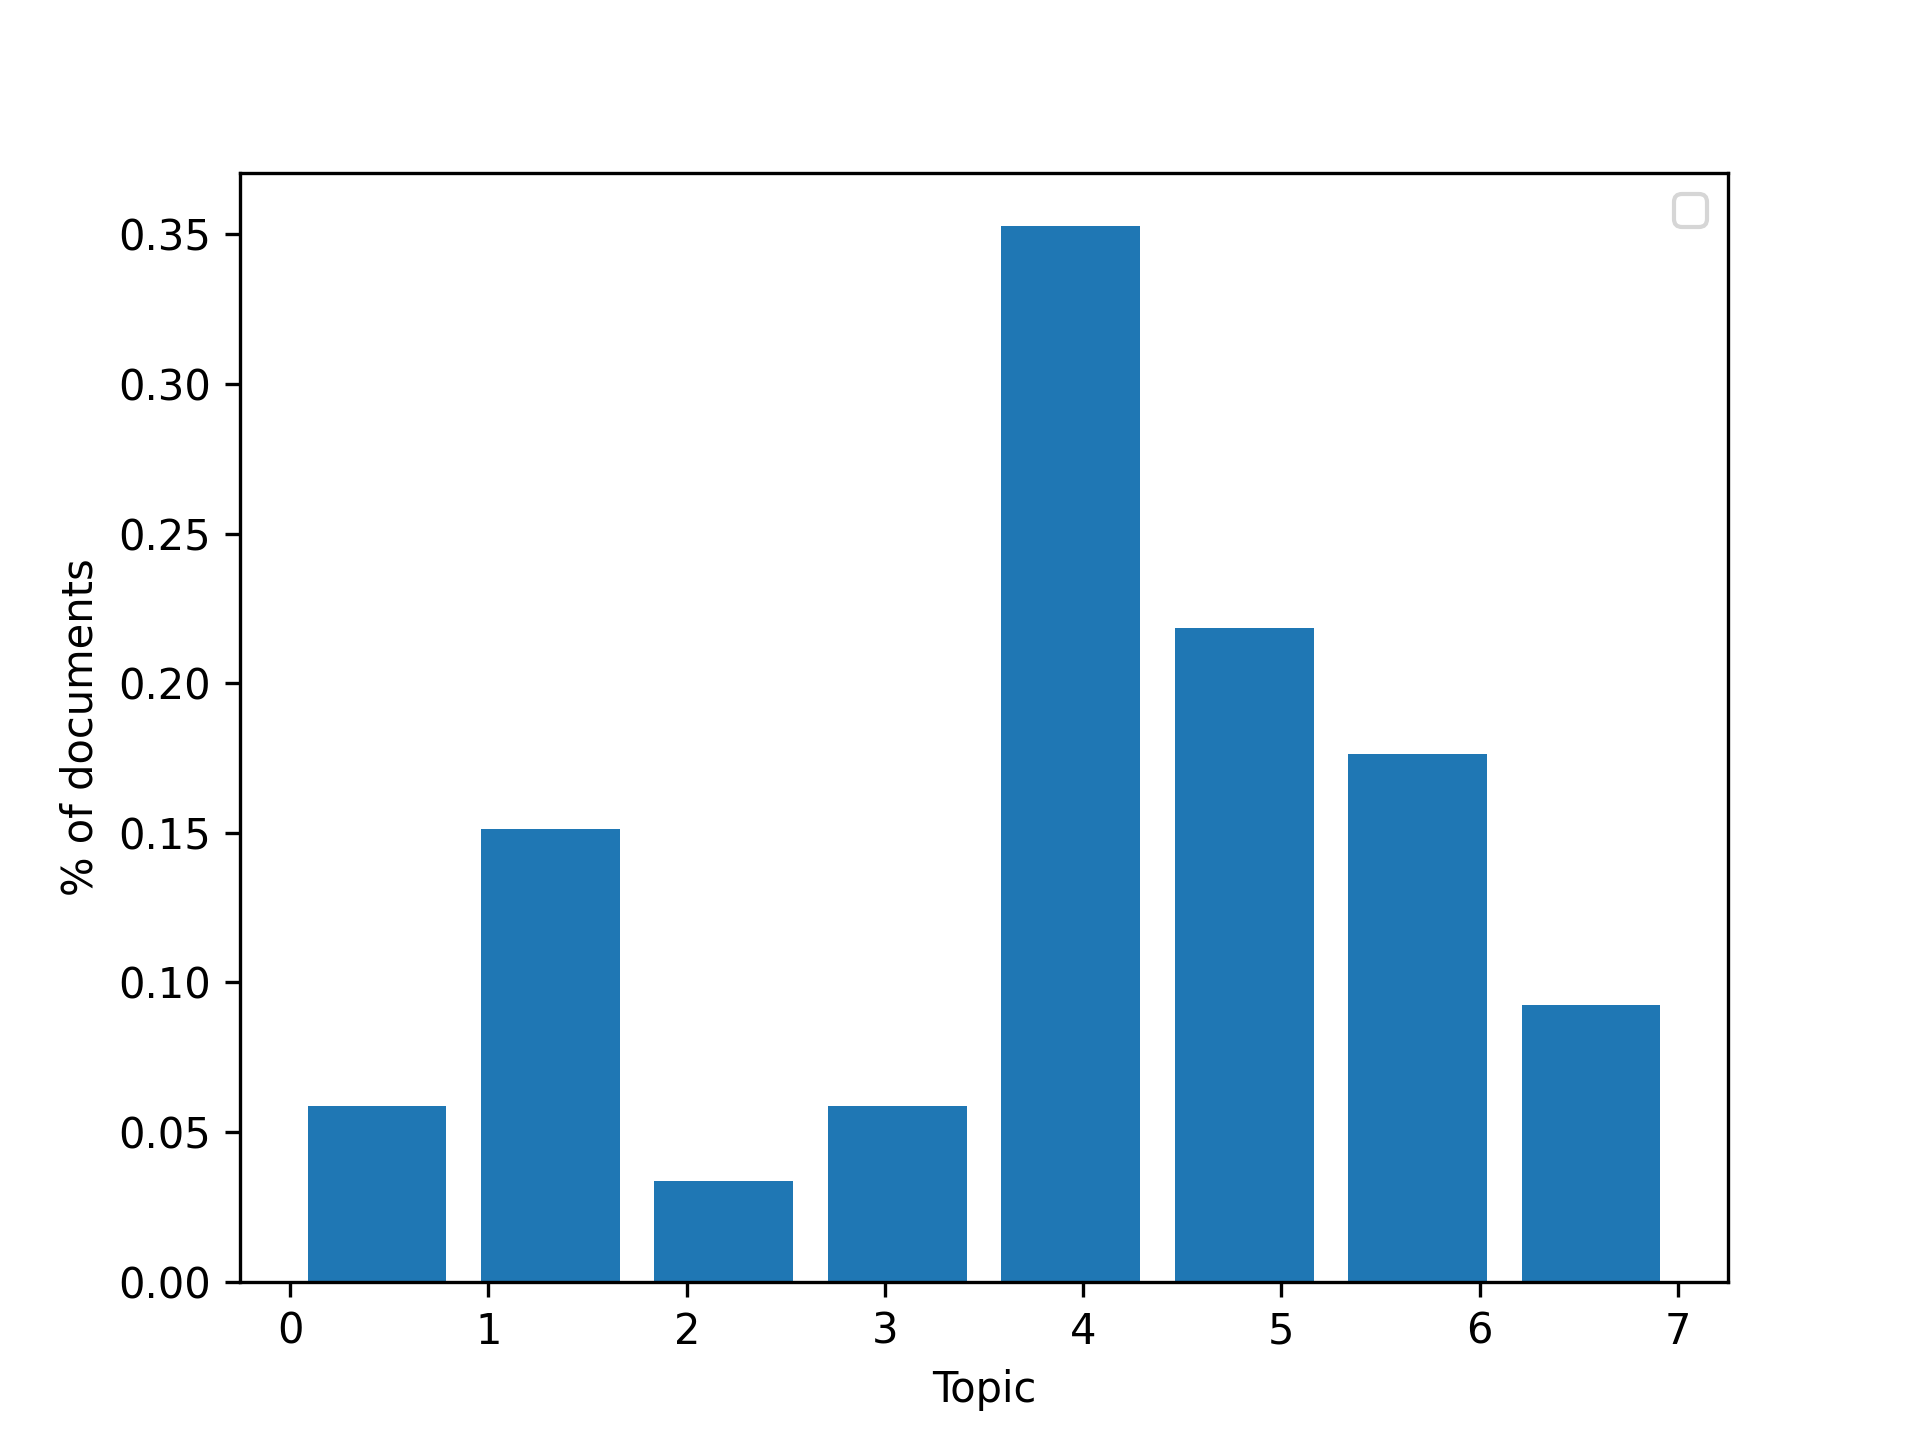
\includegraphics[width=0.7\linewidth]{topic-probabilities.png}
    \caption{Topic probability distribution of the documents in the corpus.}
    \label{fig:topic-probabilities}
\end{figure}

\section{Next steps} \label{sec:next-steps}

\subsection{Graphics APIs} \label{sec:next-steps-apis}

As we refine our statistical analyses, we then proceed to profile GPU performance of the
projects we have selected, giving special attention to those that implement
another graphics API besides CUDA.
We will then compare the performance between top projects in each category, and
analyze different implementations of similar routines.
This requires understanding the different APIs, and how they work.
It will also require finding useful benchmarks and tools and possibly
implementing our own.

\bibliographystyle{sbc}
\bibliography{references}

\end{document}
